% \documentclass[10pt,preprint,nocopyrightspace]{sigplanconf}
% \documentclass{acm_proc_article-sp}

%%%%%%%%%%%%%%%%%%%%%%%%%%%%%
\documentclass[preprint,10pt]{sigplanconf}
%%%%%%%%%%%%%%%%%%%%%%%%%%%%%

% Load basic packages
\usepackage{balance}  % to better equalize the last page
\usepackage{graphics} % for EPS, load graphicx instead 
%\usepackage[T1]{fontenc}
\usepackage{txfonts}
\usepackage{pslatex}    % comment if you want LaTeX's default font
%\usepackage[pdftex]{hyperref}
\usepackage{dingbat}
% \usepackage{url}      % llt: nicely formatted URLs
\usepackage{color}
\usepackage{textcomp}
\usepackage{booktabs}
\usepackage{ccicons}
\usepackage{subfigure}
\usepackage{authblk}
\usepackage[shortlabels]{enumitem}
%\usepackage{todonotes}
\usepackage[hyphens]{url}
\usepackage[draft]{hyperref}
\usepackage{pifont}
\newcommand{\numcircled}[1]{\ding{\numexpr191+#1\relax}}
\usepackage{multirow}
\usepackage{comment} 
\usepackage{listings}
\usepackage{xspace}

\usepackage{tikz}
\usepackage{calc}
\def\checkmark{\tikz\fill[scale=0.4](0,.35) -- (.25,0) -- (1,.7) -- (.25,.15) -- cycle;} 
\def\scalecheck{\resizebox{\widthof{\checkmark}*\ratio{\widthof{x}}{\widthof{\normalsize x}}}{!}{\checkmark}}

%that'
% llt: Define a global style for URLs, rather that the default one
\makeatletter
\def\url@leostyle{%
  \@ifundefined{selectfont}{\def\UrlFont{\sf}}{\def\UrlFont{\small\bf\ttfamily}}}
\makeatother
\urlstyle{leo}

% To make various LaTeX processors do the right thing with page size.
\def\pprw{8.5in}
\def\pprh{11in}
\special{papersize=\pprw,\pprh}
\setlength{\paperwidth}{\pprw}
\setlength{\paperheight}{\pprh}
\setlength{\pdfpagewidth}{\pprw}
\setlength{\pdfpageheight}{\pprh}
\def \theequation {\arabic{equation}}

%%%%%%%%%%%%%%%%%%%%%%%%%%%%%%%%%%%%%%%%
% Useful reviewing/feedback annotations
%\input{annotations}
%%%%%%%%%%%%%%%%%%%%%%%%%%%%%%%%%%%%%%%%

\usepackage{xcolor}

\newcommand{\todo}[1]{{\color{red}\bfseries [[#1]]}}
\newcommand{\alam}[1]{{\color{red}\bfseries [[#1]]}}
\newcommand{\TP}[1]{{\color{red}\bfseries [[#1]]}}
\newcommand{\AM}[1]{{\color{red}\bfseries [[#1]]}}
\newcommand{\rpm}{\raisebox{.2ex}{$\scriptstyle\pm$}}

% create a shortcut to typeset table headings
% \newcommand\tabhead[1]{\small\textbf{#1}}

\newcommand{\permitbreak}{\discretionary{}{}{}}

% Make sure hyperref comes last of your loaded packages, to give it a
% fighting chance of not being over-written, since its job is to
% redefine many LaTeX commands.
\definecolor{linkColor}{RGB}{6,125,233}
\hypersetup{%
  pdftitle={Syncperf},
  pdfauthor={},
  pdfkeywords={},
  bookmarksnumbered,
  pdfstartview={FitH},
  colorlinks,
  citecolor=black,
  filecolor=black,
  linkcolor=black,
  urlcolor=linkColor,
  breaklinks=true,
}

\newcommand{\spaceneedle}{\raisebox{3pt}{\includegraphics[width=6pt]{spaceneedle}}}
\newcommand{\mass}{\raisebox{5pt}{\includegraphics[width=8pt]{mass}}}
\newcommand{\texas}{\raisebox{5pt}{\includegraphics[width=8pt]{texas-orange}}}
\newcommand{\maple}{\raisebox{4pt}{\includegraphics[width=5.5pt]{maple}}}

\newcommand{\punt}[1]{}

\newcommand{\MallocProfiler}{{\texttt{maprof}}}
\newcommand{\MP}{{\texttt{maprof}}}
\newcommand{\Heapperf}{{\texttt{maprof}}}
\newcommand{\pthread}{\texttt{pthread}}
\newcommand{\pthreads}{\texttt{pthreads}}
\newcommand{\specialcell}[2][c]{%
  \begin{tabular}[#1]{@{}c@{}}#2\end{tabular}}

%\newcommand{\specificthanks}[1]{\@fnsymbol{#1}}

% \newcommand{\todox}[1]{\textcolor{red}{TODO: {#1}}}

\definecolor{lightgray}{rgb}{.9,.9,.9}
\definecolor{darkgray}{rgb}{.4,.4,.4}
\definecolor{purple}{rgb}{0.65, 0.12, 0.82}



\makeatletter
\let\@copyrightspace\relax
\makeatletter

\begin{document}

\special{papersize=8.5in,11in}
\setlength{\pdfpageheight}{\paperheight}
\setlength{\pdfpagewidth}{\paperwidth}

\title{maprof: A General Profiler for Different Memory Allocators}

\authorinfo{}
%\date{}

% Guangming Zeng will be one of the authors. 

\maketitle

\subsection*{Abstract}

MallocProfiler will be an general profiler that can be utilized to profile all types of allocators, as long as they support the same groups of memory management functions, such as malloc, free or others. 

 

%\category{D.1.3}{Programming Techniques}{Concurrent Programming--Parallel Programming} \category{D.2.5}{Software Engineering}{Testing and Debugging--Debugging Aids, Monitors, Tracing}\category{D.3.4}{Programming Languages}{Run-time environments}

\keywords
Performance, Synchronization, Multithreaded Programs, Profiling, Instrumentation


%\section*{Outline}

Introduction: 

we start with the performance data of different applications. Then we get a conclusion that allocators plays an important role in the performance of applications. 

However, there is no allocator profiler. Most existing ones are profiling the behavior of applications, but not allocator themselves. General profilers are not suitable for explaining the behavior of allocations and deallocations. For instance, perf could report the total number of cache misses, but it could not tell whether there are excessive number of cache misses on each deallocation (a significant problem of DieHarder's allocator).

\MP{} is the first general allocator profiler that focuses on multiple aspects of the allocator: performance overhead, memory overhead, scalability, and application friendliness. 

Performance overhead of each allocation and deallocation on average:
Time spent: RTDSC timestamp
Instructions inside on average: PMU
Cache misses: PMU
TLB misses: PMU

For memory overhead, \MP{} not only reports the total memory overhead, but also reports the percentage of overhead from each part, such as metadata, alignment, or memory blowup caused by using different allocators. 

For the scalability, \MP{} focuses on the scalability issues caused by software contention, typically caused by user space and kernel space contention. For user space contention,  \MP{} will report the number of locks are explicitly utilized, the number of lock acquisitions, and how much percentage of time are spending on the lock waiting inside the allocations. In addition to that, \MP{} will report the corresponding kernel contention inside the memory management: the number of times and percentage of time invoking system call, such as mmap, munmap, madvise, brk? How much time spending on kernel-space contention? 


Challenge 1: How to know the specific details of different allocators? We utilized a small program to get the allocator's specific feature. For instance, whether they are BIBOP style or Bump-pointer based, the size class information and the metadata information. 

Challenge 2: how to perform the profiling? Similar to existing work, we majorly use the time (supported by RTDSC), the number (instrumentation-based counting), and some hardware events (PMU events) to perform the sampling. The sampling approach will be similar to existing work, but we attribute those events to the memory management events, such as allocations and deallocations. 

Challenge 3: how to reduce the performance overhead? In order to reduce the number of cache contention, we re-design our data structure to avoid false sharing and true sharing as much as possible. Also, we 

Challenge 4: we propose a novel method to evaluate the application friendliness. We evaluate the cache friendliness, or TLB friendliness. 

Challenge 5: we employs an internal allocator to avoid the interfering with allocations and deallocations of applications.  


Overview:
\MP{} is an drop-in library that should be linked before any runtime library. Similar to existing profilers, \MP{} also collects  hardware events, time information and the number of invocations. However, \MP{} attribute these events or data to each invocation of memory allocation and deallocation, which can present users  intuitive information about the possible issue of each allocator. As a profiler, \MP{} further summarizes the performance overhead, memory overhead, scalability, and application friendliness of each allocator. 

  


  


\section{Introduction}

%The memory management has a significant performance impact on the performance of applications, which could lead to as large as $9.7\times$ performance difference with different allocators. Figure~\ref{fig:motivation} evaluates the performance of five applications from two popular benchmark suite, PARSEC-2.0~\cite{parsec} and Phoenix~\cite{phoenix}, with the default Linux allocator (Glibc-XXX), TCMalloc-2.2, jemalloc-4.2.0, and Hoard-3.11. The figure shows that choosing a different allocator may cause the performance difference between 32\% faster to 9.7$\times$ slower.  

The performance of modern applications is often bottlenecked by memory accesses. when obtaining undesired performance, the programmers mainly focus on optimizing the program code. Although memory allocators serve as the sole proxy for programs to request and return memory from the operating system, programmers lack even basic understandings of their behaviors, such as how well they perform themselves, how they interact with the OS, and whether their memory management policy fits the target program. 

Popular memory allocators indeed have dramatically different performance impacts on programs. Figure~\ref{fig:motivation} shows the normalized performance of ?? allocators on ?? benchmarks (details of the experimental setting in Section~\ref{sec:eval}) from two popular suites with ?? as the baseline. No allocators perform consistently the best across the benchmarks, and the largest performance gap of them on the same program is as large as ??X. For such cases, spending any additional effort of optimizing the user code will have the less impact than that of simply switching to a performance allocator.

\begin{figure}[!ht]
\centering
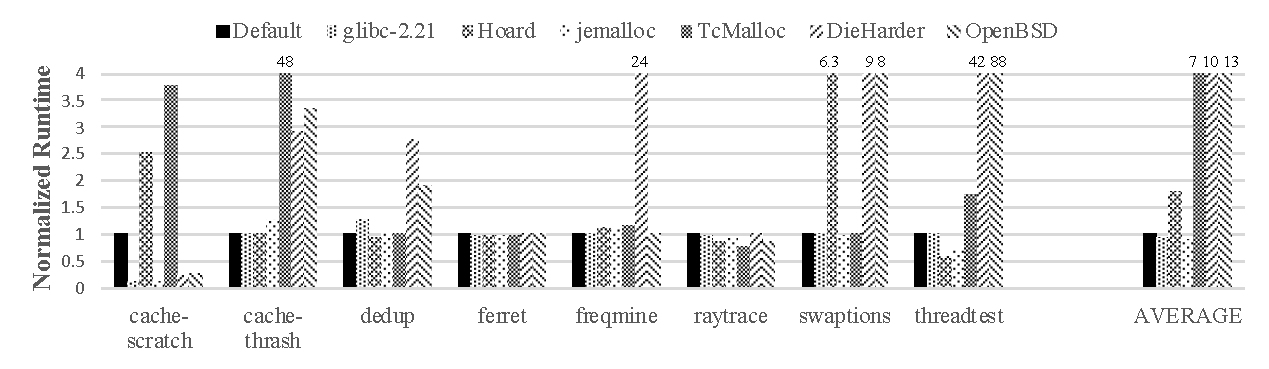
\includegraphics[width=3.3in]{figures/motivation}
\caption{Performance with Different Allocators\label{fig:motivation}}
\end{figure}

Unfortunately, there exist no profilers for the programmers to understand the behavior of memory allocators in terms of their performance impacts. Existing allocation profilers, such as \MP{}~\cite{Zorn:1988:MAP:894814}, \texttt{TCMalloc} Profiler~\cite{tcmalloc-profiler}, CLR profiler~\cite{lupasc2014dynamic} or others~\cite{hirotaka2003developing}, mainly focus on how an application uses the memory,  instead of identifying the design problems of the allocators themselves. For instance, \texttt{mprof} may attribute memory allocations based to different allocation sites~\cite{Zorn:1988:MAP:894814}. The \texttt{TCMalloc} profiler reports program sites with a large number of allocations, locates memory leaks, and reports heap usage of any time~\cite{tcmalloc-profiler}. General profilers, such as gprof~\cite{DBLP:conf/sigplan/GrahamKM82}, Coz~\cite{Coz}, and perf~\cite{perf}, can not differentiate the performance issues caused by allocators and application code. Existing studies~\cite{Barroso:1998:MSC:279358.279363, Masmano:2006:CMA:1167999.1168012, ferreira2011experimental} simply compares the performance of different allocators, without revealing the underlying reasons. 

%Facing with this vast performance difference of different allocators, programmers may want to choose an appropriate allocator for their applications, in order to maximize the performance potential. Also, when facing performance degradation, they may also want to identify whether the degradation is caused by the allocator or not. For allocators designers, it is also extremely helpful to know the underlying reason of the performance slowdown (or speedup) of a specific allocator, so that they could further augment their design. All of these targets could be satisfied with an allocator profiler.  

In this paper, we propose \MP{}, the \textbf{first} general profiler to profile different memory allocators. \MP{} uses the hardware Performance Monitor Units (PMU) and RDTSC timestamps widely available in modern CPUs to perform the profiling. \MP{} achieves three goals to act as a practical memory allocator profiler for real-world programs. First, it should directly work on the executables. Second, it should reveal the overhead and scalability of the allocators themselves. Since the invocations to the memory management functions are synchronous, the efficiency of the allocator has a direct impact on performance. Third, it should quantify the ``application friendliness'' of the memory allocator, a metric to show how well the allocator manages memory for the application, which is drawn from statistics of accesses to different levels of the memory hierarchy.

%(1) When the profiler works directly on the executable, it is difficult to distinguish the behaviors caused by the allocators and those caused by the program code. 
% TP: I removed this, since it is too trivial, but they just didn't think about it. 
We face multiple challenges to achieve the goals. (1) The profiler, despite sampling a large number of events and obtaining extensive information, should maintain a low runtime overhead, and should not seriously distort the execution of the profiled targets (e.g. allocator).  (2) The profiler should not only identify the regular design issues (e.g., poor cache locality or poor object reuses) of the allocator, but also reveal the serious issue of interacting with the OS since a poor design may invoke excessive OS system calls and introduce unnecessary kernel contention. (3) A memory allocator may significantly affect the performance of applications, not just limiting to itself, which has never been evaluated quantitively before. (4) The profiler should be able to adapt to different allocators, which is the major target of designing a general profiler.   
%  to be quantified. 
% manage memory outside of its library calls, which is hard to capture and quantify. 
%carefully manage its internal memory allocations to

To address these challenges, we design \MP{} in a principled way to determine what events to sample and what profile knowledge the sampled events contribute to. Briefly speaking, \MP{} always intercepts the allocator library calls to figure out when the program execution is inside the allocator, during which it samples both performance related PMU events (e.g., cache misses) to determine the implementation issues and intercepts OS kernel calls to understand OS-level contention. When the program execution is outside of the allocator, \MP{} samples specific PMU events to determine cache line- and page-level utilization ratio, and cache contention rate, which could directly and significantly impact the performance of the corresponding applications. To maintain low overhead, \MP{} employs a fast lookup mechanism that enables fast checking on the size information of each object, and on the cache line usage and page usage upon each sampled access. ??(WB) one more sentence about the low overhead?? ??(WB) It allocates its internal memory on ...??

\MP{} successfully identifies several implementation issues located in popular allocators. For instance, \MP{} finds out that the DieHarder allocator causes excessive number of cache and TLB misses upon each deallocation, e.g. \todo{5 times} on average compared an optimized design. \MP{} reveals that multithreaded allocators, such as ??, reclaims memory but fails to reuse these freed memory for future requests, typically from another thread, which causes the blowup problem~\cite{Hoard}. \MP further shows that the ??allocator invokes different system calls, such as \texttt{mmap}, \texttt{brk}, \texttt{madvise}, and \textbf{munmap}, which cause unnecessary kernel contention inside the OS (and limit its scalability). Lastly, \MP{} evaluates the application friendliness of the allocators and show that the program's poor performance when using ?? is strongly correlated with its low friendliness. In all the profiling runs of real-world programs using popular allocators, \MP{} incurs at most ??X runtime overhead ??X memory overhead, while sampling and processing a large amount of events, and for the first time revealing various performance issues latent in the allocators.

%Basically, \MP{} utilizes the hardware Performance Monitor Units (PMU), RDTSC timestamp, and simple counters together to perform the profiling. For instance, it utilizes the RDTSC timestamps to collect the execution time of each allocation/deallocation, and utilize simple counters to obtain some statistics information, e.g. the number of allocations and deallocations, and so on. It also employs PMUs to collect  hardware events of each allocation and deallocation, such as TLB read/write misses, retired instructions, and page faults. Different from existing work, \MP{} proposes \textbf{the novel usage of PMUs to evaluate application friendliness}, such as cache utilization (and contention) ratio and page utilization ratio, which may indirectly affect cache misses and TLB misses. \MP{} samples memory accesses, and then obtains the cache utilization ratio and page utilization ratio in which each sampled access is located, and utilizes the sampled ratio to represent the overall ratio. Therefore, \MP{} could quantify the potential performance impact of a specific allocator on applications.    

However, there exists multiple implementation challenges. The most important challenge is the \textbf{overhead challenge}, where one careless design may impose up to 100 $\times$ overhead, based on our experience of the development. The huge overhead could be unaffordable even for development phases. More importantly, the significant overhead may skew the evaluation results unnecessarily. \MP{} takes multiple approaches to reduce the performance overhead. First, \MP{} designs a fast lookup mechanism that enables the fast checking on the size information of each object, and on the cache line usage and page usage upon each sampled access quickly, as further discussed in Section~\ref{sec:fastlookup}. This lookup mechanism is very difficult to design, since different allocators may have different behaviors, and their memory mappings are out of the control of \MP{} (without some obvious rules). Second, \MP{} minimizes the cache contention by utilizing thread-local recording, and only summarizing the data together in the end of execution. Third, \MP{} also reduces the allocation overhead of its recording data structures, by preallocating the space for internal memory usage. For instance, it employs the vast address space of 64-bits machines to design its lookup mechanism, and pre-allocates a huge space for saving the mapping. 

Another significant challenge comes from the adaption to different allocators. Specific issues include the following ones: (1) How to obtain the specific details of different allocators, such as size class information, type of allocator, metadata size information? (Section~\ref{}) (2) How to design the fast but general lookup mechanism for different allocators (Section~\ref{})? There are multiple factors may affect the design: the default Linux allocator extends its heap differently with the \texttt{sbrk} system call, making one of its heap arena far from other arenas (making it difficult to design the virtual memory)? Secure allocators, such as OpenBSD and DieHarder, may invoke one \texttt{mmap} to obtain one page from the OS. That is, there are a large number of mappings inside the OS. This fact makes some general data structures not suitable to support the fast lookup, such as a hash map or the range tree. (3) How to measure the kernel contention inside the OS (Section~\ref{})? The Linux's glibc-2.21 has a very serious performance problem that is caused by the kernel contention, due to its careless invoking of system calls (\texttt{madvise}). (4) How to measure the user-space contention for the Glibc's allocator (Section~\ref{})? 

\begin{comment}
Challenge 2: how to perform the profiling? Similar to existing work, we majorly use the time (supported by RTDSC), the number (instrumentation-based counting), and some hardware events (PMU events) to perform the sampling. The sampling approach will be similar to existing work, but we attribute those events to the memory management events, such as allocations and deallocations. 

Challenge 3: how to reduce the performance overhead? In order to reduce the number of cache contention, we re-design our data structure to avoid false sharing and true sharing as much as possible. Also, we 

Challenge 4: we propose a novel method to evaluate the application friendliness. We evaluate the cache friendliness, or TLB friendliness. 

Challenge 5: we employs an internal allocator to avoid the interfering with allocations and deallocations of applications.  

 
\MP{} utilizes multiple methods to minimize the performance overhead of the profiling.  

\end{comment}

\MP{} also avoids the pollution on the profiling data. For instance, since \MP{} is designed to profile the allocators on specific applications, its internal memory allocations should be separated from those  of applications. \MP{} avoids the change of different allocators by intercepting allocations/deallocations and system calls through the preloading mechanism, which makes it a drop-in library. Overall, \MP{} only introduces around $2\times$ performance overhead and around $3\times$ memory overhead, while providing abundant information about allocators itself. During its experimentation, \MP{} is employed to discover various issues of existing popular allocators. It further presents the first quantitative comparisons on different allocators, not limiting to the external performance comparison on different applications.  

%\MP{} is also adapted to different allocators, which employs a  test program to obtain the details of different allocators, such as the type of the allocator, size class information, and the metadata overhead of each object. 


\begin{comment}

1. Maybe we should detect the contention rate. If the last write is from a different thread, we will detect one contention. 
 
allocator: can we use some different configurations of the same allocator?
Can we use the same allocator on different applications, achieving different allocators?  
}





performance overhead: 
1. Using the hash maps to identify the size of each object is very slow. 
2. Turning multiple reads into one read around 2 or three times. 
3. Using the new mapping mechanism. 

How we can do that for glibc. We migrate the glibc as separate library, allowing us to intercept system or libraries. 

How to figure out the metadata information?
	
\end{comment}

 



\begin{comment}

Challenge 1: How to know the specific details of different allocators? We utilized a small program to get the allocator's specific feature. For instance, whether they are BIBOP style or Bump-pointer based, the size class information and the metadata information. 

Challenge 2: how to perform the profiling? Similar to existing work, we majorly use the time (supported by RTDSC), the number (instrumentation-based counting), and some hardware events (PMU events) to perform the sampling. The sampling approach will be similar to existing work, but we attribute those events to the memory management events, such as allocations and deallocations. 

Challenge 3: how to reduce the performance overhead? In order to reduce the number of cache contention, we re-design our data structure to avoid false sharing and true sharing as much as possible. Also, we 

Challenge 4: we propose a novel method to evaluate the application friendliness. We evaluate the cache friendliness, or TLB friendliness. 

Challenge 5: we employs an internal allocator to avoid the interfering with allocations and deallocations of applications.  


Overview:
\MP{} is an drop-in library that should be linked before any runtime library. Similar to existing profilers, \MP{} also collects  hardware events, time information and the number of invocations. However, \MP{} attribute these events or data to each invocation of memory allocation and deallocation, which can present users  intuitive information about the possible issue of each allocator. As a profiler, \MP{} further summarizes the performance overhead, memory overhead, scalability, and application friendliness of each allocator. 


For performance overhead, \MP{} focuses on the following items: 


Since memory overhead can be caused by multiple factors, such as metadata overhead, alignment overhead (internal fragmentation), and memory blowup. Memory blowup is defined as ,. 

For scalability, \MP{} not only focuses on the potential bottleneck within the user space, but also includes the potential bottleneck caused by the allocator. Programmers have identified one particular performance bottleneck of applications, such as dedup issue. 
It won't cause the . 

\MP{} also aims to answer whether an allocator is friendly to the applications or not, such as . . 


   


MallocProfiler will serve two purposes. 
(1) This will be utilized to get the allocator related parameters. 

(2) We will be able to identify whether the performance problem is caused by the memory allocator. We could actually divide the overhead to the overhead of allocator or the overhead of applications. 
Therefore, we could identify the root causes and not always blame for the application writer. 



 

However, the memory allocator itself has not got sufficient attention that it should reserve to. 
For instance, there is no an dedicate the allocator profiler that can be utilized for identify the allocator's behavior.

Having this profiler will serve three purposes. First, it will help the designers and developers that could discover the issues of memory allocators, without the need of porting or developing the profiler for a specific allocator. Second, it helps programmers to determine whether the performance issue is coming from the memory allocator. Third, it will help users to choose the best memory allocators that is suitable for a specific applications, if there are multiple choices available. 

 Linux, TCMalloc, Jemalloc, Hoard, OpenBSD, DieHarder. Then shows the internal reason of why some are slower than others. 

We may choose two general-purpose allocators and two secure allocators. Then we know why secure allocators are slower, currently. 

The general idea is to understand performance, memory, and scalability of different allocators, while providing some evidence of allocator. During the design of allocator, we usually need to understand the inherent reason. The difficulty is how to collect the information without changing the specific allocator. That is, how to design a general allocator profiler, which can help assist the analysis of different allocators. 

We will work on the allocator profiling to understanding the performance, memory and scalability of memory allocator. We may  memory related those system calls. How long it spent on the memory allocation and deallocation, using RDTSC, which can be caused by long memory allocation time? How much of objects has been re-utilized? How is the memory blowup, what is the memory consumption and how much has been allocated? Can we know lock contention of memory allocation, maybe we could monitor the lock usage, just as SyncPerf, and identify that lock acquisitions are  waiting during allocation? Can we identify is there inter-objects cache contention on these objects? If yes, that is the possible example of these allocators.  

What are the design goals of \MP{}? 

\MP{} needs to be general to different memory allocators, which requires no change of the code at all even when connecting with different allocators. The first target is transparency, which should not require the changes of allocators, if the allocator is working as a dynamic library. 

Second, \MP{} should be able to identify the issues of different allocators. 


	
\end{comment}


\begin{comment}

Dynamic memory management plays an important role in the performance of applications, especially on multithreaded programs. 
For performance related to memory uses, some work focuses on improving existing memory allocators. Some focuses on a better memory layout among different elements of the same data structure. 
But there is little work that focuses on the improving the performance by changing the behavior of memory allocations and deallocations. 

\HeapPerf{} tries to identify some places inside applications that can introduce the performance problems. These problems can be solved by changing the behavior of memory allocations, without using the new memory allocator. 
These problems are rarely investigated in the past. The most closest work related to this is to simply record the placement with excessive allocations. However, excessive allocations is a total class of the problems that are investigated in this paper, but the existing work fails to present any detailed idea on the following problems: whether all these excessive memory allocations can be reduced? whether they can improve the performance? how to reduce that? These questions requires highly expertise and large amount of manual effort. Instead, \HeapPerf{} presents more useful idea on these questions, and hope to guide programmers, even non-experts, to solve these problems easily. 

We observe three different patterns that can cause performance problems, or called as anti-patterns~\cite{}. 

The second type is shown as Figure~\ref{}. In this example, there are a number of memory allocations that will allocate small amount of bytes for each one. More particularly, these allocations are inside the same loop, and have the same size. Unfortunately, memory allocators will not precisely allocate the specified size of objects. For example, the \texttt{glibc} allocator will allocate 32 bytes as long as the required size is between 4 bytes and 24 bytes. Based on the explanation of Hoard~\cite{Hoard}, this method helps to manage small sizes of different objects, without introducing too many external fragmentation. However, this also introduces a significant problem on cache inefficiency, since only less than 13\% cache is actually utilized, which can introduce around $8\times$ performance slowdown comparing to the code listed in Figure~\ref{}. 


The second type is shown as Figure~\ref{}, there are a number of unnecessary memory allocations and deallocations. By moving the placement of allocations to outside the loop, we can significantly improve the performance by reducing the overhead related to memory allocations and deallocations. 

The third type is related to the uses of heap variables or stack variables. Some excessive heap objects, if they are turned into stack variables, will have large performance benefit. Comparing to heap objects, the overhead of memory allocations and deallocations can be largely reduced if using stack variables. Also, the stack is typically locate inside the cache, which will have lower access latency. Also, stack variables will have exact size, without the addition of metadata and huge alignment. 
\todo{Whether those variables have been touched only very few times, typically should be putted into the heap objects since they may cause the in-efficient cache utilization as well}.  
 


Heap memory related performance bugs can be from the following categories, if only think about applications. 

\begin{itemize}
\item: Too many allocations and deallocations. The total run time spending in memory allocation and liberation may take up to 30\% execution time\cite{1190248}. 

\item: Too many memory uses: this can actually affect the performance when there are too much memory that has been allocated but not used. This can be caused by memory leaks or too late de-allocation. \todo{Most existing tools focus on the memory leak, but whether there are some tools that can uncover delayed-deallocation?}  

\item: 
\end{itemize}


What we can do for heap memory management?

First, we can point out the unnecessary memory allocations and deallocations. For example, we can malloc a large object, and then assign to different small projects. Some of them may be called inside the internal level of loop functions, we can move up to external loop level. 
By reducing unnecessary memory allocations, we expect to improve the performance. 

Second, we can give a statistics on the life-span of objects. Whether we can find out some problems inside? For example, we can use stack variables instead of heap if some objects are too short-lived, or mostly inside a function call. 

Third, we can actually give the statistics on each callsite. Some callsites may have larger number of allocations. 

Can we evaluate the performance related to heap allocations? For example, how much time is spending on memory allocation. 
We can approximate the time of spending on each allocation. Then we can attribute the time to different statements, just similar to gprof. Then maybe it is obvious that we can reduce the overhead by reducing the memory allocations. Then it is possible that a separate paper by using the 


In the end, although not every interested, it is to check the overhead of every memory allocation on each popular memory allocation. Thus, pointing out that the memory allocation actually should pay attention to the level of stacks. Thus, it is possible that we can design a new memory allocator by reducing the level of memory allocation. This is a reverse to HeapLayer. It is great to have an survey paper on this:

A. How is the overhead of memory allocation in large applications? How we can evaluate it? 
B. How is the overhead that comes from memory management? We evaluate this on some popular benchmarks. 
C. Whether the overhead comes from different cache uses? or other things. 
D. It will shed a light whether we need to re-design the memory allocator. 
It will be a perfect paper for ICSE or SC.

How we can evaluate the cache friendliness of memory allocators? 
For instance, how much memory will be reutilized immediately? If one direct use will be one point, then how many score of different allocators. 

Also, how much of memory blowup? 

%%%%%%%%%%%%%%%%%%%%%%%
% Possible solutions:
% (1) We will check the malloc and free are allocated in sequence. For example, we are always doing the malloc(8) and free(8) in sequence. Given the number of these allocations is large. Then it is much possible that it is a problem. However, it can be a problem for the performance reason. But we can basically maintain a stack that maintains five possible allocations. 
%% Should we just use a two-phase solution? That is, we can use a hash-table to identify different allocation site with their memory uses: how many times for memory allocations? How many times for related free operations? If there are a lot of memory allocations that are not freed, then it is possible a memory leak. We could also identify whether those memory are actually touched or not by using the watchpoint mechanisms? Also, we may try to check whether memory allocation are in the same sequence, for example, alloc-free-alloc-free, and with the same size. If yes, then it is possible that is unnecessary memory operations. 

%%%%%%%%%%%%%%%%%%%%%%%%%
Typically, I think that mtrace utilizes 

Can we check the example of malloc-free situations?
Can we base on a ``anomaly detection'' but.  
I guess that the memory will be freed before the next allocation. If not, then there is high probability of leaking. If memory allocated is on the same site, 
	
\end{comment}
 

\subsection*{Contribution}

Overall, this paper makes the following contributions. 

\begin{itemize}
\item It designs and implements \textbf{the first general profiler}--\MP{}--to profile different aspects of different memory allocators, without changing allocators themselves.  

\item \MP{} employs advanced hardware, such as Performance Monitoring Units (PMU) or Read Time-Stamp Counter (RDTSC), and simple counters together to profile allocators quantitatively. \MP{} attributes the data to each allocation and deallocation, helps discover some issues that cannot be discovered with general profilers.  
%Overall, it can not only pinpoint the major issues inside the implementation of memory allocators, such as performance, memory, and scalability issues, but also could quantitively pinpoint cache or page utilization issues of allocators.  

%\item \MP{} proposes the employment of hardware PMUs to evaluate performa metrics efficiently and effectively. 

\item This paper performs extensive experiments on multiple memory allocators. It pinpoints some performance or memory issues latent in existing allocators. It also provides the first quantitative comparison of different factors of multiple widely-used allocators.  

\end{itemize} 

\subsection*{Outline}

The remained of this paper is organized as follows. Section~\ref{} discusses the overall design purpose of \MP{}, and Section~\ref{} presents the detailed implementation. Section~\ref{} shows the results of experiments on different allocators using \MP{}. Then Section~\ref{} discusses related work in this field, and Section~\ref{} concludes this paper. 
\section{Overview}

\MP{} is designed as a drop-in library that can be simply linked to applications (and allocators), without the requirement of changing the code or even re-compilation. Although \MP{} could employ the binary-instrumentation to perform a more detailed profiling, such as identifying the instructions within each allocation or deallocation, the binary instrumentation may impose prohibitive performance overhead. With a high overhead, the profiling results may be significantly skewed, such as the waiting time of each lock acquisition inside the allocation. Instead, \MP{} employs the PMU hardware, RDTSC timestamp hardware, and simple counters together to perform the profiling.  
 
As described above, \MP{} focuses on two aspects of the allocator, the allocator itself and its potential impact on applications (application friendliness). In order to adapt to different allocators, a small program is designed to collect the allocator's specific feature, such as the type of allocators, the size class information, or others. 

In the remainder of this section, we describe the profiled items for each category, and the basic idea of profiling. 

\subsection{Background of Allocators}

\label{sec:allocator}

There exists multiple types of allocators, such as bump-pointer, BIBOP, and region-based allocators. However, region-based allocators are only suitable for special situations that all allocated objects within the same region can be efficiently deallocated at once~\cite{Gay:1998:MME:277650.277748}, which is not the common type for popular allocators. Based on the common knowledge,  the number of requests for small objects is significantly much larger than the number of big objects. Thus, most allocators utilize different mechanisms to manage ``small'' and ``big'' objects, where the bump-pointer and BIBOP style typically indicates their mechanisms to manage small objects. For big objects, allocators may map a block of memory from the OS directly during an allocation, and then return it to the OS via \texttt{munmap}~\cite{Hoard}.   

\textbf{Bump-pointer} allocators typically utilize a  arithmetic operation to bump a pointer when the block is first allocated~\cite{Cling}, in which objects with different sizes can be allocated adjacently. Freed objects are typically placed into different free lists, based on their size classes.  Therefore, they typically have to get the size information of each object upon deallocations. Since objects with different size classes are placed continuously, it will be slow to look up the size information if placed in other placements (no way to compute). Therefore, the size information is typically placed on the header of objects to support the fast look up.  Two examples of this type are the Glibc allocator, the default allocator in Linux that originates from dlmalloc~\cite{dlmalloc}, and Hoard~\cite{Hoard}.  

The \textbf{BIBOP} allocators belong to another common type of allocators, where the BIBOP stands for '' Big Bag of Pages''~\cite{hanson1980}. For these allocators, one or multiple continuous pages are treated as a ``bag'', holding objects with the same size class. The metadata of heap objects, such as its size and availability information, is typically stored in a separate area. Thus, BIBOP-style allocators improve the security and reliability, by avoiding metadata corruption caused by buffer overflows. Many performance-oriented allocators, such as TCMalloc~\cite{TCMalloc}, \texttt{jemalloc}~\cite{jemalloc}, and most secure allocators, such as OpenBSD~\cite{OpenBSD} and DieHarder~\cite{DieHarder}, belong to this type. BIOBP allocators may utilize free lists or bitmaps to manage the availability of objects. When using the bitmap, only one bit metadata is sufficient to track the availability of an object, which may impose less memory overhead for the metadata but with possibly higher performance overhead.  


Almost all existing allocators manage objects by  size classes, instead of the exact size of objects. But different allocators support  different size classes: some only support power-of-2 sizes, such as DieHarder~\cite{DieHarder} or the OpenBSD allocator~\cite{OpenBSD}, while some utilize more fine-grained size classes, such as the Glibc allocator and jemalloc~\cite{jemalloc}. For each allocation request, the allocator will round up the requested size to the nearest size class. Upon each deallocation, the deallocated object will be threaded into the corresponding free list (for the freelist design) or the corresponded bit will be cleared (for the bitmap design). Therefore, the idea of size class enables the re-use of heap objects. However, it may introduce \textit{internal fragmentation}, wasting the space between the actual allocated size and the size class. 

In order to support multithreaded applications, most allocators typically support per-processor heap design, one idea introduced by Hoard~\cite{Hoard}. For instance, Hoard maintains per-processor heaps and a global heap concurrently. Allocation requests from different threads typically will be satisfied from different per-processor heaps, avoiding false sharing and reducing the lock contention at the same time. Thus, this design actually augments the scalability of allocators. However, it may introduce the \textit{memory blowup}, one typical issue existing in multithreaded allocators. Based on our understanding and experiments, the memory blowup is the one major reason why different allocators may impose different physical memory consumption. 

\subsection{Basic Idea of maprof}
\MP{} profiles different types of data as discussed in the following. 
  
\subsubsection{Performance Overhead}

For performance overhead, \MP{} profiles the average data of each allocation and deallocation, instead of the summarized values over the whole execution. Per allocation/deallocation data helps identify internal issues inside, if the data is counterintuitive. For instance, \texttt{DieHarder} is identified to have a very high number (\todo{up to X}) of cache misses upon each deallocation, which clearly a deficiency. 

First, \MP{} collects the time spending on each allocation and deallocation. It intercepts allocations and deallocations of allocations, and then computes the RDTSC timestamp difference of before and after each operation as the execution time. The allocation and deallocation time is a very important metrics on the efficiency of an allocator.  

%TLB read misses/TLB write misses/page faults/cache misses/instructions. They are PMU-based. 
% 

Second, \MP{} further collects hardware PMU events for each allocation and deallocation, where the introduction of PMU is described in Section~\ref{sec:pmu}. The PMU events allow \MP{} discover the specific information of allocations/deallocations without the instrumentation, such as retired instructions, cache misses, and TLB read/write misses. 

%Based on our understanding, the hardware events, such as retired instructions, cache misses or TLB misses, will help reveal some implementation issues of an allocator. For instance, \MP{} detects that the DieHarder allocator has an excessive number of cache misses and TLB misses upon each deallocation, around 5 times of each deallocation, which is significantly larger than that of other allocators. By examining the code, we found out a serious implementation issue of the DieHarder allocator, which traverses all mini-heaps to identify the placement of each object. Obviously, this implementation is extremely slow, considering that every deallocation has to perform such expensive lookup. By fixing such issues, the DieHarder's performance improves around \todo{20\%}.     


\begin{comment}
Can we integrate the cache misses or page faults for each allocation and deallocation, so that we could identify the issue of DieHarder that invokes many unnecessary cache misses?

If we could correlate cache misses to each thread, then we could do this. 

If allocation and deallocation takes too much time, it could be caused by multiple reasons:

(1) First, it just takes a lot of instructions (could we find out the lapsed instructions for each thread?)
(2) It may be caused by not good algorithm? 
(3) It can be caused by lock contention?
(4) It can be caused by system call related contention?
\end{comment} 

\subsubsection{Memory Overhead}

Based on our understanding, the memory overhead of each allocator comes from three aspects: the metadata overhead, the alignment (or internal fragmentation), and the memory blowup. 
How much memory are due to memory re-utilization rate? For instance, we may not fully utilize the memory due to the randomization mechanism. We only care about physical memory waste. Then we should also investigate how much memory has been explicitly returned back to the OS. 

How much memory are due to the metadata itself? 

\subsubsection{Scalability Analysis} 

User space contention:
How many separate locks are explicitly utilized? 
How many lock acquisitions? How much time are spending on lock waiting for each thread, and in total?

How much time spending on kernel-space contention? For instance, we could infer from memory-related system calls, such as mmap, munmap, madvise, brk, or something else? 

That is, we may have to integrate with SyncPerf for doing this. We will borrow their implementation in order to do this. 

\subsubsection{Application Friendliness} 
How many page faults and cache misses that are caused by applications? 

How many remote accesses? How many interconnect messages? We may employ the PMU mechanism to identify the information.

\subsection{Technical Challenges}

As described above, \MP{} employs hardware PMU, RDTSC, and simple counters together to perform the profiling. Also, as described above, there are some challenges. 
 

How to support the default Linux allocator, since it actually utilizes some internal function calls, which cannot be intercepted by \MP{} normally. Therefore, we actually migrated its allocator as a separate library, as other allocators. This allows \MP{} to intercept all lock acquisitions, system calls as usual. 

How to track the size information of objects for both bump-pointer allocators and BIBOP allocators? We observe that it is difficult to track the range of objects. In fact, we also utilize the ?

How to know the metadata overhead of each allocator? It is very difficult to identify which region is used to save the allocator information, without changing the source code of the allocator. Also, it is even difficult to know. We observe that the allocator overhead comes from multiple aspects: metadata overhead, alignment overhead (or internal fragmentation introduced by size classes), and then memory blowup. 
As far as we know the total memory overhead, then the metadata overhead = total heap size - alignment overhead - memory blowup overhead - memory usage.

However, if the allocator itself utilizes the global variable or an pre-allocated block as the metadata, which can be omitted by \MP{}. 

 


\subsection{Background of Performance Monitoring Units}
\label{sec:pmu}

\subsection{Background of RDTSC}

\label{sec:rdtsc}







\section{Design and Implementation}
\label{sec:implementation}

This section discusses the implementation and design of \MP{}. To profile an allocator, \MP{} intercepts memory allocations/deallocations, memory-related system calls, and synchronizations. This also indicates that an allocator should utilize standard APIs in order for \MP{} to collect corresponding information. However, the Linux allocator utilizes the internal implementation of synchronizations by default. For the profiling purpose, it should be changed to invoke explicit POSIX-APIs instead. Fortunately, most allocators do not need any change or the recompilation.  \MP{} profiles the performance, memory overhead, scalability, and application friendliness, as discussed in different subsections. 

 %It also discusses some common issues, such as adapting to different allocators, and the performance issue of collecting data. 

\subsection{Profiling Performance Data}

\label{sec:performanceimplement}

\MP{} profiles the performance overhead of every memory management operation. Since an allocator typically has different execution paths for different scenarios (as discussed in Section~\ref{sec:allocator}), such as new or re-used allocations, small or big objects, \MP{} further collects the information for each scenario separately. The fine-grained data helps identify a particular design issue inside. For instance, DieHarder has a serious performance issue for deallocating small objects for \texttt{dedup}, with 744105 cycles and 2.8 cache misses for each deallocation. However, it has the similar number of cycles and deallocation runtime  for deallocating big objects. Given the fine-grained data, programmers could only focus on the deallocation path relating to small objects.

\MP{} collects the allocation data for small objects and large object separately, where small objects further include new and re-used allocation. For deallocation, \MP{} collects the deallocation data for small and big objects separately. \MP{} collects the average runtime of each allocation and deallocation with the RDTSC instruction (Section~\ref{sec:pmu}), due to the performance and accuracy reason. Time stamps are taken before and after each operation, and then the difference between them is the runtime of an operation. 

\MP{} differentiates the types of an operation as follows. To differentiate small and big objects, \MP{} relies on a configuration file as further described in Section~\ref{sec:understandingallocators}. It is also important to differentiate between new and re-used allocations, since they typically have over $20\times$ performance difference on average. \MP{} uses a global hash map to assist this differentiation: every allocated object will be inserted into the global hash map in its allocation time, and will be kept in the table; If an allocation is found to be in the hash map, then this allocation is a re-used allocation. Otherwise, it is a new allocation.  


\MP{} also employs the PMUs to collect hardware events of each operation, such as cache misses, page faults, TLB misses, and instructions. These hardware data are  significant supplements for identifying an issue, given that \MP{} is a non-intrusive profiler that cannot know the implementation details of an allocator. Let us revisit the issue of DieHarder. DieHarder is found to have a large number of cycles for its deallocation. However, it is difficult to know the particular issue inside, if without more information. An unusual number of cache misses for each deallocation helps identify the design issue: DieHarder traverses all bags one by one to determine the original bag for an allocation, causing excessive number of cache misses. Similarly, \MP{} collects hardware events before and after each operation, and uses the difference of two counters as the number of events occurring inside an operation. 

\subsection{Profiling Memory Overhead}
\label{sec:profilingmemory}

For memory overhead, \MP{} reports the ratio of different types of memory overhead, such as internal fragmentation, memory blowup, and other memory overhead, and real memory usage. Therefore, programmers can pinpoint memory consumption clearly. We have described the concepts of different types of overhead in Section~\ref{sec:memoryconsumption}. However, it is challenging to collect corresponding data correctly and efficiently.


Conceptually, internal fragmentation is the difference between the size class and the requested size for a small object. However, if the difference is larger than a page, the internal fragmentation cannot be computed  with this method. We need to consider page allocation policy, where the OS only allocates a physical page if it is used. Based on this, internal fragmentation for such objects should be adjusted correspondingly: for a new allocation, the fragmentation will be difference between the end of the object and the end of its last page; For a re-used object, \MP{} should track the maximum pages of this object, and use the difference between the end of its last page and the end of the object as internal fragmentation. When an object is released, its internal fragmentation should be decremented. \MP{} utilizes the same hash map as described in Section~\cite{sec:performanceimplement} to track the maximum pages for each object. 

It is challenging to compute memory blowup correctly. By the definition of Section~\ref{sec:memoryconsumption}, a new allocation will be treated as memory blowup, if there exist freed objects for this size class in freelists of other threads. However, this definition does not specify whether memory blowup should be reduced upon deallocations, and what to do if such objects are re-allocated again. \MP{} computes memory blowup based on the following observation: \textit{all freed objects of a size class is the upper bound for its memory blowup.} Then, \textit{the upper bound deducted by the size of recent freed objects is memory blowup}. This definition is intuitive, since recent freed objects are not belonging to memory blowup, since they will exist anyway. Based on this definition, \MP{} further implements a practical method to compute the number of recent objects. The intuitive method is simply using a global counter to track recent freed objects for each size class. The counter is incremented upon every deallocation, but will be decremented upon each allocation only when the counter is larger than 0.


In addition, it is very expensive to frequently collect all data, when memory consumption reaches its maximum value. Therefore, \MP{} only updates the data periodically, when the total memory usage is increased by 1MB. Also, it is also very expensive to update all data using global counters, since that will cause significant cache contention. Therefore, \MP{} tracks most of data using thread-local variables, and then summarizes all data together when reaching the maximum memory consumption. \MP{} only uses global variables for the memory consumption and the counter of recently-freed objects. But even with these two global variables, it is expensive to update them with the full synchronization or even atomic variables. Instead, \MP{} updates these variables without synchronization primitives or using atomic variables, which may loose some updates. But \MP{} should still provide a reliable percentage for different types of memory overhead, based on our evaluation.  

%these data,  real memory usage is the amount of memory actually requested by the application, where real allocated memory is the sum of real memory usage and internal fragmentation due to size-class based allocation. For example, if an application requests the memory by \texttt{malloc(454)}, then real memory usage is incremented by $454$, but real allocated memory will be incremented by the size of its corresponding class size. For this example, total memory will be incremented by page size instead (e.g., 4096 bytes), provided that the page was previously unused. 



%\MP{} also collects different types of memory overhead, such as internal fragmentation, memory blowup, and others. It also collects the available memory and total memory consumption of each size class. The detailed data help programmers to pinpoint its memory overhead issue. For instance, if memory overhead mainly comes from the internal fragmentation, then the allocator should utilize more fine-grained size classes. If the memory overhead mainly comes from memory blowup, the allocator may require to adjust its synchronization frequency or take a more aggressive method for its synchronization~\citep{DBLP:conf/iwmm/LiLD19}. The memory overhead could be reduced with coalescence or splitting, if the major memory overhead comes from external fragmentation. 

%\MP{} typically records different counters upon each allocation and deallocation. For the performance reason, \MP{} typically maintains a per-thread counter in order to reduce the contention issue. The per-thread counters includes the number of allocations and deallocations for each size class, the number of bytes for internal fragmentation, and allocated objects for each size class. \MP{} utilizes a global hash table to track the status information for each object, Therefore, \MP{} could adjust the internal fragmentation upon each deallocation. 



% \MP{} reports other memory overhead as a summarized value, including external fragmentation, metadata overhead, and explicitly skipped objects. It is difficult to differentiate them without the implementation details. %Since \MP{} traps all memory usage requested by the allocator, the remaining memory except internal fragmentation and memory blowup will be reported. 
 

 
 %External fragmentation occurs when an allocator has sufficient memory but in a non-continuous way. Therefore, \MP{} keeps a global counter for the available memory, so that it could determine whether an allocation causes the external fragmentation issue or not.  The counter for the memory blowup will be incremented, if the current per-thread heap has no freed objects but there exit freed objects with the requested size class in other per-thread heaps. Therefore, \MP{} maintains a global counter for each size class. 

% Upon an allocation request, if the current thread does not possess any freed objects of the given size class -- but if the global counter does -- we record this event as an allocation responsible for increasing the allocator's memory blowup.

  
%  \todo{Based on the definitions of memory blowup and external fragmentation, an allocation will be counted as a memory blowup if there exists freed objects with the same size class. However, it is difficult to evaluate the external fragmentation. For instance, if freed objects with smaller class sizes exist, with the total size larger than the requested size, then the current allocation should be counted as external fragmentation. However, if freed objects with larger class sizes exist, it should not count as external fragmentation. But the overhead is caused by the issue of size class or without-splitting. Maybe we should make it clear in Section 3.3. }     
 

\subsection{Profiling Scalability}
\label{sec:profilingscale}

\MP{} also collects the scalability data of a memory allocator. As described in Section~\ref{sec:scalability}, \MP{} evaluates the scalability for both user space and kernel space. 

For user-space scalability, \MP{} mainly collects the number of acquisitions, the runtime of each acquisition (with the RDTSC instruction), the runtime of each critical section, the number of contentions, and the number of maximum contending threads. \MP{} utilizes RDTSC instruction to collect the runtime. The challenging part is to track the contention information, without re-implementing synchronizations. \MP{} dynamically maintains the contention state of each lock. Before the acquisition, \MP{} increments the contention threads of the corresponding lock, which will be decremented upon the release of this lock. \MP{} utilizes a hash table to track the status of every lock. In theory, the contention data is not very accurate, since increments and decrements are not atomic. However, the data could still show the contenting status of locks inside an allocator.    

For the kernel-space scalability, \MP{} focuses on memory-related system calls inside the allocation and deallocation, including \texttt{mmap}, \texttt{munmap}, \texttt{mremap}, \texttt{sbrk}, \texttt{madvise}, and \texttt{mprotect}. \MP{} profiles the runtime of each invocation with the RDSTC instruction, and the number of invocations for each system call. In order to identify the issue of a specific execution path, \MP{} also collect the data for each type of allocations and deallocations, similar to the performance overhead of Section~\ref{sec:performanceimplement}.
In fact, the simple data could actually uncover serious scalability issues of a memory allocator. For instance, the Linux allocator of \texttt{glibc-2.21} slows down an application by 20\%, which can be uncovered by the excessive number of \texttt{madvise} system calls and a higher runtime for the corresponding \texttt{mmap} and \texttt{mprotect} system call. 


\subsection{Application Friendliness}
\label{sec:profilefriendliness}

%Currently, the Linux kernel has supported PMUs starting from 2009 (Linux-2.6.31)~\cite{pmulinuxsupport}, where users could set up performance monitoring via  the \texttt{perf\_event\_open} system call. After collecting events, the user program could fetch these events. 

\begin{comment}
Cache line utilization: 
Shadow memory. 
Cache line: real using memory.
page: real used memory.

False sharing: 
Lines:
Cache contention rate: owner, if the current write operation is not the existing owner, we will increment the counter. 
We will report the percentage with write. 

False sharing, 
active/passive: 
how many lines with active and passive. 
	
\end{comment}

 
For application friendliness, \MP{} focuses on the following metrics, including cache/page utilization rate, cache contention rate, and false sharing effect. \MP{} employs PMUs to sample memory accesses periodically, with a default sampling period of 100,000. Then \MP{} updates these metrics upon every sampled access. \MP{} employs the shadow memory to track the information, in order to compute these values. 

For cache and page utilization rate, \MP{} maintains the number of used bytes for the  the current cache line and the current page, which will be updated on each allocation and deallocation. Upon every sampled event, \MP{} increments the number of cache lines and pages that have been accessed, and also increments the counter to track the total number of bytes on this cache line. In the end, \MP{} computes the utilization rate with a simple division. For cache utilization rate, the dividend is the total number of used bytes, and the divisor is the the total number of bytes for these cache lines. The page utilization rate is computed similarly, but focusing on the page level instead. 

However, the challenge is to quickly locate the  metadata for each cache line and each page, since the metadata should be updated upon every allocation and deallocation, and upon every sampled event. During its implementation, \MP{} has tried multiple mechanisms. First, \MP{} designed a red-black tree to hold memory mappings of the heap, and then stored the address of corresponding metadata on the tree node. This mechanism was found to be in-efficient, since some allocators (e.g., OpenBSD) includes thousands of mappings, which may introduce tens of comparisons unfortunately. Second, \MP{} utilized a hash map to store the memory mappings. But it is difficult to decide the right number of buckets for the hash table, where a small number may cause too many conflicts, with significant performance overhead by traversing the link list.  Finally, \MP{} designs a fast lookup mechanism by taking advantage of the vast address space of 64-bits machines, where the detailed design is discussed as follows. 

% Based on our observation, all allocators invoke either \texttt{sbrk} or \texttt{mmap} system calls to obtain the memory from the underlying OS. The address range returned from \texttt{sbrk} is generally lower than 4G, while the range returned by \texttt{mmap} is typically less than 128TB. 
%Given that modern processors typically support 48 bits address space (256 TB), \MP{} employs the last TB (between 255TB and 256TB) of address space to store the meta data of object, with the design illustrated in Figure~\ref{fig:lookup}. 

\textbf{Three-Level Fast Lookup Mechanism:} \MP{} designs a three-level lookup mechanism as illustrated in Fig.~\ref{fig:lookup}, borrowing the idea of multi-level page table design of OS. Basically, a ``MB Mapping'' will be the first level, where the index can be computed simply by dividing an address with 1 megabytes (MB). Each entry of this MB mapping points to all possible pages inside the current 1-megabyte memory. Since one MB memory will have at most 256 pages, with the size of 4KB for each page, each MB entry points to 256 page entries. Similarly, each page entry has the information about used bytes in this page and has a pointer pointing to 64 possible cache entries inside. Based on this design, it takes two steps to get the used bytes for a page, and takes three steps to get the used bytes for the current cache line. Therefore, it has the $\mathcal{O}(1)$ 
complexity to obtain the metadata.  
          
\begin{figure*}[!h]
\centering
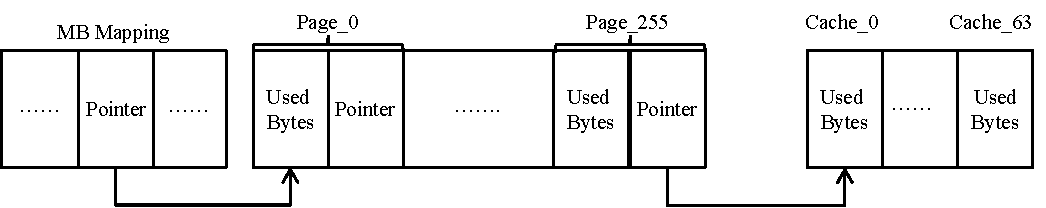
\includegraphics[width=5.5in]{figures/lookup}
\caption{Three-level Lookup Mechanism.\label{fig:lookup}}
\end{figure*}

Note that this design is also efficient in memory consumption. If a range of addresses are not used, then there is no need to allocate physical memory for the corresponding page entries and cache entries. This design is able to adapt to different allocators, where memory mappings of a heap is varied from a few to hundreds of thousands, and these mappings can be scattered along the whole address space of a process. 
%To track valid memory mappings dynamically, \MP{} intercepts memory related system calls inside allocations/deallocations, such as \texttt{sbrk}, \texttt{mmap}, \texttt{munmap}, \texttt{mremap}. 

For false sharing effect, \MP{} focuses on two aspects: the number of cache lines that has false sharing, either active or passive false sharing, and the number of cache contention events on these cache lines. Identifying active and passive false sharing is relatively intuitive based on the definition, by checking the number of threads in each cache line. We employ three-level lookup table as discussed above to store the threads information that are allocated from the same cache line. 
For cache contention events, \MP{} relies on sampled memory accesses. Upon each sampled event, \MP{} checks whether the event is a write access. For each write, \MP{} updates the last thread to write on the corresponding cache line to be the current thread. If the current thread is different from the recorded last thread, \MP{} increments the number of cache contention events. In the end, \MP{} reports the percentage of cache contention on identified cache lines with false sharing issue. 

\MP{} also reports the number of cache contention events on cache lines without active/passive false sharing issues, using the same method. In fact, cache contention events on these cache lines can be caused by internal-object false sharing or true sharing, but they cannot be solved with a different memory allocator. However, the reported data could help understand whether an application is running slow or not. Note that \MP{} is not designed to be false/true sharing detection tool. If \MP{} reports a big cache contention rate, users may resort to specific tools to identify specific issues inside the application~\cite{Sheriff, Predator, DBLP:conf/ppopp/ChabbiWL18}. 
   

\subsection{Predicting Performance Impact}
\label{sec:predict}

In order to help users determine whether an allocator is the culprit of the performance issue, \MP{} further predicts the potential performance improvement after switching to  a better allocator. Predicting the performance impact is very complicated, since an application can be affected by multiple factors, such as hardware/software  contention and synchronization. From the point view of an allocator, it can be affected by both cache friendliness and memory management overhead. \MP{} only focuses on the latter one, which provides an lower bound on the potential improvement. Basically, \MP{} replaces the runtime of memory management operations with a standard runtime, and then predicts the reduction of the total runtime.  

For the standard runtime of every memory management operation, \MP{} utilizes the median values collected from a range of applications. Basically, based on our evaluation, the default Linux, TcMalloc, and jemalloc are three best allocators in terms of the performance. Then we choose the best allocator for each application in terms of cycles for each memory management operation, and then select the median value for each operation. Note that there are different choices to choose the standard runtime for every operation, and we only utilizes a simple one to proof the concept. We have thought about that the runtime of a memory management operation can be related with the parallelization and the frequency of allocation. However, it is challenging to build a direct relationship based on our evaluation results. For instance, a serial allocation can also take tens of thousands of cycles. 

To predict the runtime reduction, \MP{} further collects the runtime outside memory management operations with the RDTSC instruction. 
     

\subsection{Adapting To Different Allocators}
\label{sec:understandingallocators}

\MP{} is designed as a general profiler for sequential and BiBOP-style allocators, as described in Section~\ref{sec:allocator}. The challenge is to adapt  to different allocators. \MP{} interprets a configuration file to identify the difference of every allocator in its initialization phase, such as the allocator's style (BiBOP-style versus sequential), sizes of different classes, the threshold of separating small objects from large objects. This configuration can be provided manually. \MP{} also provides a prerun program to understand these details of an allocator. 

In order to identify the style of allocator, the prerun routine will check whether two subsequent allocations with different sizes (small objects, apparently from different size classes) are allocated from the same page or not. If yes, then the allocator is a sequential-style allocator, which is similar to the default Linux allocator. Otherwise, the allocator belongs to a BiBOP-style allocator. 

The second step is to identify the sizes of different size classes. The prerun routine begins by allocating an object of 8 bytes, and continues to allocate additional objects using a stride increase of 8 bytes each time. The determination of size classes depends on the style of an allocator. For BiBOP-style allocators, an allocation with a different size class will be satisfied from a different bag, locating in a different page. For sequential allocators, such as the Linux allocator, we employ the \texttt{malloc\_usable\_size} to  return the bag size for an allocation with the specified size. 

%the distance between two contiguously-allocated objects (with distinct sizes) is utilized to determine the size class. As shown in Fig.~\ref{fig:sizeclass}, if the size of $Obj_1$ and $Obj_2$ is the same, judging from the distance of between two continuous objects, then they belong to the same size class. Otherwise, they belong to different size class, such as $Obj_3$ in the figure. By checking the size of two objects belonging to different objects, we could determine the sizes of different size classes.  
\begin{comment}

\begin{figure}[!ht]
\centering
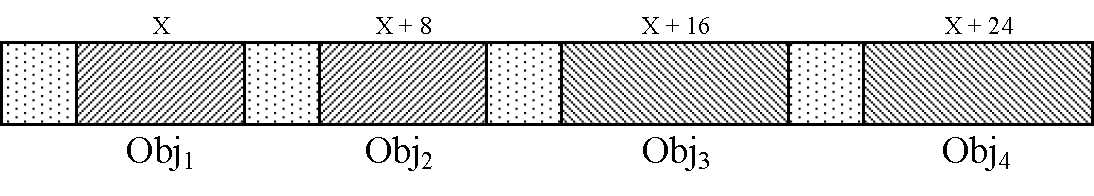
\includegraphics[width=5in]{figures/sequentialclasssize}
\caption{Determining the size class of a sequential allocator by the distance between continuous allocations. \\The boxes with 10\% dotted pattern are the metadata, and the boxes with diagonal stripes\\ are actual heap objects. The number above every box is the size of the corresponding object. \label{fig:sizeclass}}
\end{figure}
	
\end{comment}


The threshold for big objects are typically detected by checking whether there is an explicit \texttt{mmap} system calls upon the allocation. Typically, most allocators utilize a direct \texttt{mmap} system call to satisfy the allocation for a big object initially. However, this threshold requires the manual confirmation. 


\section{Experimental Evaluation}
\label{sec:evaluation}

This experimental evaluation will answer the following questions:
\begin{itemize}
\item What is the effectiveness of \MP{}? (Section~\ref{sec:effectiveness}) 	
\item What is the performance overhead of \MP{}? (Section~\ref{sec:perf})
\item What is the memory overhead of \MP{}? (Section~\ref{sec:memory})
\end{itemize}

Experiments were performed on a two-processor machine, where each processor is Intel(R) Xeon(R) Gold 6230 and each processor has 20 cores. This machine has 256GB of main memory, 20MB of L2 cache, and 1280KB L1 cache. The underlying OS is Ubuntu 18.04.3 LTS, installed with the Linux-5.3.0-40. All applications were compiled using GCC-7.5.0, with \texttt{-O2} and \texttt{-g} flags.

\subsection{Effectiveness}
\label{sec:effectiveness}

In order to evaluate the effectiveness, we evaluate \MP{} with five widely-used allocators, including two versions of the Linux allocator (versions 2.21 and 2.28), TCMalloc~\cite{tcmalloc}, jemalloc, and Hoard, and two secure allocators, i.e. DieHarder and OpenBSD. These allocators include both sequential and BiBOP-style allocators. Secure allocators were included, since they have their unique memory management policies. 

For the evaluation, we use the default configurations of these allocators. However, we make some changes in order to  intercept synchronizations. Since the Linux allocators are included within the \texttt{glibc} libraries, they invoke the internal synchronizations (\texttt{lll\_lock}) directly, which cannot be intercepted by \MP{}. They are thus recompiled separately as a stand-alone library for the purposes of evaluation. Because Hoard is using \texttt{std::lock\_guard} for its synchronization, we replaced these with POSIX spinlocks to track its synchronization behavior.

%\todo{Let's use a table to list all dramatic difference between these allocators. This gives us some evidence of allocators}
%\subsection{Issues Identified in Different Allocators}

\begin{comment}

\begin{table}[h]
  \centering
  \caption{Abnormal metrics of allocators for different applications.\label{table:abnormal}}
  \footnotesize
  \setlength{\tabcolsep}{0.2em}
\begin{tabular}{l | l | l | l | l}
\hline
Applications & Allocator & Behavior & Abnormal Metrics & Root Cause \\ \hline
cache-thrash & TcMalloc & $47.7\times$ slowdown & Contention rate for PFS lines: 50\% & Root Cause \RN{1} \\ \hline
dedup & glibc-2.21 & 20\% slowdown &  \# of Madvise for small allocations: & Root Cause \RN{2} \\ \hline
freqmine & jemalloc &  Memory consumption & memory blowup: 2174230K (37\%) & Root Cause \RN{3} \\ 
 & &  & external fragmentation: 1132045K (19\%) \\ \hline
swaptions  &  DieHarder  & $9\times$ slowdown  & 
	Small reused alloc: 377476 cycles 	& Root Cause \RN{4} \\
& & & Small free: 331745 cycles, and 4.9 cache misses & \\ 
& & & Per-lock acquisition: 353448 cycles & \\\cline{4-5}
& & & External fragmentation: 1878K(37\%) & Root Cause \RN{5} \\
& & & cache utilization 55\%, page utilization 35\% & \\\cline{2-5}
& Hoard & $6.3\times$ slowdown & 
	Small reused alloc: 68933 cycles, 9.4 cache misses 	& Root Cause \RN{6} \\
	
& & & Small free: 53402 cycles, 11.8 cache misses & \\ 
& & & 1.54 locks per-operation & \\
\cline{4-5}
& & & Memory blowup: 4789K( 81\%) & Root Cause \RN{7} \\
& & & cache utilization 62\%, page utilization 51\% & \\\cline{2-5}
& OpenBSD & $8\times$ slowdown & Small re-used alloc: 98962 cycles, 4.5 cache misses & Root Cause \RN{8}\\ 
& & & Small free: 101081 cycles, 7 cache misses & \\ 
& & & 1.1 locks per-operation &  \\ \hline
  \end{tabular}
\end{table}
\end{comment}


%issues of allocators that were detected by \MP{}.
%The detailed data reported by \MP{} will be presented in order to show the helpfulness of its report. 

\paragraph{TcMalloc:}
%TcMalloc typically performs very well in almost all applications, except \texttt{cache-thrash} and  \texttt{cache-scratch}. For instance,
TcMalloc runs $38\times$ slower than the default allocator for \texttt{cache-scratch}. \MP{} reports the runtime of allocations and deallocations of TcMalloc, which is at a normal range. But it reports around a 22\% cache invalidation rate for passive false sharing issues, which is the major reason causing the significant slowdown.  
%TcMalloc actually experiences both active and passive false sharing issues. For active false sharing, TcMalloc will get one object for a thread from its central heap each time, so that two continuous objects can be utilized by two different threads. Since 
Based on our understanding, TcMalloc always places a freed object to the current thread's per-thread cache, which may introduce passive false sharing that two objects in the same cache line are accessing by different threads. 
%In comparison, the Linux allocator always returns an object back to its original arena, avoiding passive false sharing.  
%TcMalloc also has 8\% internal fragmentation and 8\% external fragmentation for \texttt{swaptions}, which explains that why it has more memory overhead than other allocators. 

\paragraph{glibc-2.21:}  For \texttt{dedup}, glibc-2.21 has a known bug that may invoke excessively large number of \texttt{madvise} systems calls under certain memory use patterns~\cite{madvise}. \MP{} reports 505241 \texttt{madvise} invocations in 8.6 seconds, and the runtime of each \texttt{madvise} is about $12266$ cycles (much higher than the normal one). \texttt{madvise} introduce high kernel contention with page faults and memory-related system calls. Changing the threshold of shrink\_heap reduces the runtime from 8.6 seconds to 6.9 seconds (with 20\% improvement).

%\MP{} also reports 52\% memory wastes caused by memory blowup for this application. That helps explain why glibc-2.21 are using 740 MB more memory than TcMalloc.  

%\paragraph{jemalloc:} jemalloc typically has good performance, but has a greater memory consumption caused by both memory blowup and external fragmentation. For \texttt{freqmine} application, jemalloc has 43\% memory wastes caused by blowup. That helps explain that why it consumes 40\% more memory than TcMalloc, and 38\% more than glibc-2.21. In comparison, TcMalloc only has 2\% memory wastes and glibc-2.21 has 7\% memory wastes.  

\paragraph{DieHarder:} DieHarder runs $5.75\times$ slower than the default Linux allocator for \texttt{swaptions}. This application reflects multiple design issues of DieHarder. First, \MP{} reports an abnormally high amount of cache misses for each deallocation (around 112). Based on our investigation, DieHarder checks all miniheaps to identify the original location of an object, which introduces multiple cache misses due to the checking on multiple miniheaps. Second, \MP{} reports that DieHarder has one lock acquisition per allocation and five lock acquisitions per free operation, with 44\%  and 47\% lock contention rate for small and big allocations. The data helps explain that  DieHarder utilizes a global lock, which is certainly not scalable.  

%\textit{Root Cause \RN{5}}: we also notice that DieHarder introduces external fragmentation, around 37\%. As described before, this also includes the size of skipped objects, which is caused by DieHarder's over-provision allocation mechanism. Since DieHarder will also randomly choose some objects, that is maybe the cause of its low cache utilization and page utilization. 


\paragraph{Hoard:} 
For \texttt{swaptions}, \texttt{Hoard} is running around $2.07\times$ slower than the default allocator. \MP{} reports abnormal lock information related with medium-size objects (between 256 bytes and 8K bytes): it acquires 1.9 locks per new allocation, 1.73 locks per re-used allocation, and 2.73 locks per free operation. 
%These operations also incur 14\%, 18\% and 14\% lock contention separately. In addition to that, \MP{} reports that the average cycles of each lock is more than 400 cycles, which is much more than 30~70 cycles for the serial phase. 
Multiple locks per operation is caused by Hoard's hash mechanism: ``we use a simple hash function to map thread id’s to per-processor heaps....., there is not a one-to-one correspondence between threads and processors''~\cite{Hoard}. Because multiple threads can be mapped to the same heap, Hoard has to introduce a lock to protect each heap, which is different from TcMalloc and jemalloc's per-thread buffer. 

In addition to that, \MP{} further reports abnormal lock contention rate for some locks, up to 87\% for new allocations and 47\% for re-used allocations in parallel phase. Therefore, we utilized the debugger to identify the reason: Hoard has a threshold (defined in hoardThresholdFunctionClass) for returning a super-block back into the global pool of super-blocks based on the emptyness. Unfortunately, one deallocation could cause the current super-block to be placed into the global pool, while the next allocation will move the super-block back to the thread-local buffer. That is, the back-and-forth of moving the super-block introduces high contention on the lock of protecting the super-block pool. We changed the threshold from 64K to 4K to reduce the migration, where this single change improves the runtime from 26.17 seconds to 12.76 seconds. \textit{This is a new bug that is never reported elsewhere}. 

%Also, its overhead of using many levels of templates cannot completely go away, since Hoard has a lot of code like this: SmallHeap::malloc(), or getHeap().malloc(), Heap::malloc(). Based on our evaluation on an application (canneal) with a big number of allocations, the allocation cycles for a new allocation for Hoard will be around 520 cycles, which is 2.8X of TcMalloc (180 cycles). The cycles for a re-used allocation will be 187 cycles, which is 2.3X times of TcMalloc (83 cycles). The number of instructions is also multiple times more than TcMalloc.

%Hoard also has 40\% memory wastes for \texttt{swaptions}, where 26\% is from its external fragmentation.  
 
%\paragraph{OpenBSD:} \textit{Root Cause \RN{8}:}  OpenBSD has $8\times$ slowdown for \texttt{swaptions}, comparing to the default allocator. Based on its report, we find out that OpenBSD has the similar issue as Hoard, since it acquires more than one lock for each operation. By checking the code, we find out that OpenBSD has the same global lock for all allocations and deallocations, which is the possible reason for its big slowdown. Also, OpenBSD also has a big cache misses for its re-used allocations and deallocations for small objects, which is possibly another reason why it has a big slowdown. For OpenBSD, we also observe that it has significant big number of instructions than other allocators, which as 430 instructions for deallocating a small object, and 295 instructions for a re-used allocation. This is possibly another reason for its big slowdown. 

%\paragraph{jemalloc:}
%During evaluation, the \texttt{reverse\_index} benchmark was found to perform approximately 21\% slower when paired with \texttt{jemalloc} versus the default Linux allocator. Upon inspection, we find that, with \texttt{jemalloc}, the program exhibited over $2x$ the number of CPU cycles associated with the deallocation execution path, as well as a 34\% increase in critical section duration (i.e., the cycles spent within outermost critical sections).




 
\begin{comment}
\renewcommand{\arraystretch}{1.5}
\begin{table}[!ht]
  \centering
   \caption{Important   Metrics\label{tab:metrics}}
  
    \begin{tabular}{l|l|l|l}
    \hline
\multirow{5}{*} {Performance} & \multirow{3}{*}{Allocation Runtime} & New Allocation  (Small) & 80\\ \cline{3-4}
& & Reallocation  (Small) & 1000 \\ \cline{3-4}
& &  Large Allocation & 1000 \\ \cline{2-4}
& \multirow{2}{*}{Deallocation Runtime} & Small  &  \\ \cline{3-4}
& & Large & 100 \\ \cline{1-4}
    
    \end{tabular}
\end{table}
	
\end{comment}

\subsubsection{Observations for Allocators:} 

We have some observations on commonalities of a performant allocator. 

\paragraph{Synchronization:} It is better to reduce lock usages for an allocator. For instance, TcMalloc and jemalloc utilize per-thread cache to store objects, so that there is no need to acquire a lock if an allocation can be satisfied from a per-thread heap. Hoard, although with its per-thread heap design, actually can be slowed down a lot via its hashing mechanism. The other two counterexamples are OpenBSD's allocator and DieHarder. They both use the same lock to manage different size classes, which is one most important issue for their big slowdown. 

\paragraph{Active/Passive False Sharing:} TcMalloc although with the good performance, but it has very serious both active and passive false sharing. This could significantly slowdown the performance, even if it has almost the fast allocation/deallocation speed.  

\paragraph{Cache Misses:} Some allocators, such as DieHarder, Hoard, and  OpenBSD, have multiple cache misses per operation. That could sometime be the reason for their slowdown. The opposite for them is TcMalloc and jemalloc that always have fewer cache misses. We believe that this issue can be reduced with a better design, such as with better metadata design.  

\paragraph{Kernel space synchronization:} Kernel contention is actually very common based on our evaluation. We could observe this from the runtime of memory related system calls.  However, it is sometimes difficult to evaluate its potential impact.

\paragraph{Fine-grained size:} The Linux allocator is the only allocator has very fine-grained size, where two continuous size classes only have the difference of 16 bytes. This mechanism may impose less internal fragmentation. However, it will has the issue of external fragmentation. Although the Linux allocator also can coalesce and split objects to reduce internal fragmentation, it will pay some additional performance cost. That is the reason why the Linux allocator is typically slower than TcMalloc for most applications.

\paragraph{Re-used allocations and deallocations of small objects:} Based on our observation these two aspects are the most important to the  performance of applications, due to its large number. This is also the fast path, which should have less conflicts and fewer instructions.  


%For a performant allocator, what's the common things within the average allocator. We could utilize a table to list the average points of each allocator. Potentially, we could utilize these parameters to evaluate a new allocator. 

%For evaluating purpose, we could provide two information, one is the average with all evaluated allocators, another one is to omit one allocator with the lowest scores. 


%It seems that BIBOP style allocators are the trend of allocators, which not only has a better performance overhead on average, but also has better safety by separating the metadata from the actual heap. 



\subsection{Performance Overhead}
\label{sec:perf}

\begin{figure}[!ht]
\centering
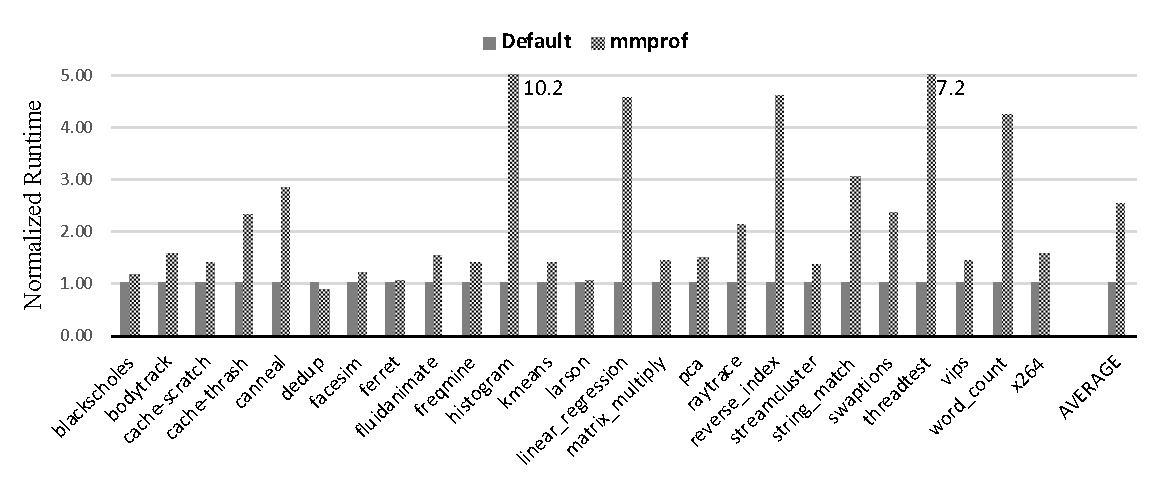
\includegraphics[width=\columnwidth]{figures/perfoverhead}
\caption{Performance overhead of \texttt{mmprof}, normalized to the runtime of default Linux allocator.\label{fig:overhead}}
\end{figure}

We evaluate the performance overhead of 
\MP{} using PARSEC~\cite{parsec},  Phoenix~\cite{phoenix}, and synthetic applications from Hoard~\cite{Hoard}. The performance overhead can be seen in Fig.~\ref{fig:overhead}, which is the average runtime of five executions. From this figure, we can see that \MP{} runs $2.6\times$ slower than the default allocator, where two applications (\texttt{histogram} and \texttt{threadtest}) impose over $5\times$ performance overhead. Based on our understanding, both the number of memory operations and the number of lock acquisitions can significantly impact the performance overhead. To help the explanation, we further collect the characteristics of these applications, as shown in Table~\ref{table:characteristics}.  

First, if an application invokes extensive applications and deallocations in a short period of time, then \MP{} may introduce a large performance overhead. For each memory operation, \MP{} invokes two RDTSC instructions to collect the runtime, updates multiple counters, and updates the state in the global hash table. Second, the number of lock acquisitions inside memory operations could also significantly affect the performance. Similarly, \MP{} also collects the runtime data of each lock acquisition via the RDTSC instruction, and update different counters. 
Since \texttt{canneal} invokes 11 million memory operations and 0.3 million locks acquisitions per second, and \texttt{threadtest} has 6 million memory operations and 33 lock acquisitions per second, that explains why these applications have a large overhead with \MP{}.  

\texttt{histogram} and \texttt{linear\_regression} are two exceptions, since they have a small number of allocations. For these two applications, \texttt{histogram}'s execution time is 0.12 seconds and \texttt{linear\_regression} is 0.3 seconds. \MP{} has an initialization phase to perform the initialization, and an finalization phase to analyze the data and write out results to the external file, which may add more overhead than a program's execution time. 
%For instance, \texttt{histogram} only takes 0.12 seconds to finish. Therefore, \MP{} adds more overhead than the program's execution time.  has the same issue, with the total execution time of 0.3 seconds.  
%for some tiny applications like \texttt{histogram}, which only takes 0.1 second when running along, \MP{}'s initialization and conclusion would take more time than themselves. Thus, performance overhead ratios for tiny applications could be larger.
%\texttt{threadtest} actually imposes more performance overhead, due to the reason that most memory opeations are actually 



%some applications invoke allocations intensively and almost simultaneously from different threads, \MP{} may introduce more contention in the hash table when checking every object's status, and higher contention rates would cause programs' slowdown.
\begin{comment}
For example, according to \ref{sec:memory}, 
canneal 2.86x   11438194.73 (alloc+free)/sec    42282925 alloc+free 311044.69 lockacqs/sec
reverse_index 4.59x 973245.43 (alloc+free)/sec 40000387 alloc+free 120407.33 lockacqs/sec
threadtest 7.21x 6 228 715.40 (alloc+free)/sec 256000203 alloc+free 33 239 532.98 lockacqs/sec



For example, according to \ref{sec:memory}, 
linear_regression 4.56x, 0.3s when running alone, 2 alloc+free
word_count 4.26x, 1.71s when running alone, 481 alloc
histogram 10.23x, 0.12s when running alone, 4 alloc+free

Upon every allocation and deallocation, \MP{} collects the runtime and acquisition information.

\end{comment}

\begin{table}[h]
  \centering
  \caption{Characteristics of applications\label{table:characteristics}}
  \footnotesize
  \setlength{\tabcolsep}{0.2em}
\begin{tabular}{l|c|r|r|r|r}
\hline
\multicolumn{1}{c|}{Application} & 
\multicolumn{1}{c|}{Runtime}    & 
\multicolumn{1}{c|}{New Alloc}     & 
\multicolumn{1}{c|}{Reused Alloc}     & 
\multicolumn{1} {c|}{Free}     & 
\multicolumn{1}{c}{Lock Acqs} \\ \hline
  blackscholes & 16.7 & 8 & 1 & 7 & 11 \\ \hline   
   bodytrack & 8.5 & 20150 & 460616 & 480765 & 871397 \\ \hline    
   cache-scratch & 3.0 & 44 & 400000 & 400043 & 47 \\ \hline    
   cache-thrash  & 2.4 & 43 & 3999960 & 4000002 & 45\\ \hline  
   canneal & 29.4 & 8756242 & 12385221 & 21141462 & 9144714 \\ \hline    
   dedup & 12.7 & 3384984 & 683368 & 1750378 & 4864027 \\ \hline    
   facesim & 159.2 & 953143 & 3955049 & 4094483 & 1678963 \\ \hline    
   ferret & 25.3 & 149680 & 236867 & 415914 & 417370\\ \hline    
   fluidanimate & 12.3 & 229912 & 1 & 229913 & 307124 \\ \hline    
   freqmine & 20.2 & 1810 & 4 & 1070 & 15926 \\ \hline    
   histogram & 0.12 & 2 & 0 & 2 & 3 \\ \hline    
   kmeans & 16.4 & 200691 & 533 & 200579 & 303705 \\ \hline    
   larson & 15.1 & 2408955 & 33726797 & 36095750 & 38088835 \\ \hline   
   linear\_regression & 0.3 & 1 & 0 & 1 & 2 \\ \hline    
   matrix\_multiply & 4.8 & 83 & 0 & 82 & 85 \\ \hline    
   pca & 9.2 & 16131 & 29 & 72 & 16466 \\ \hline    
   raytrace & 41.1 & 5000115 & 15000100 & 20000172 & 5000240 \\ \hline   
   reverse\_index & 1.5 & 1632810 & 106173 & 1738982 & 1806110\\ \hline  
   streamcluster & 23.5 & 47 & 8798 & 8844 & 17622\\ \hline    
   string\_match & 0.6 & 8 & 0 & 7 & 10 \\ \hline    
   swaptions & 14.5 & 2040 & 47999756 & 48000385 & 48002039\\ \hline    
   threadtest & 7.7 & 1280122 & 126720000 & 128000081 & 255944404\\ \hline    
   vips & 6.5 & 8128 & 1420072 & 1428019 & 1526404\\ \hline    
   word\_count & 1.7 & 481 & 0 & 0 & 481\\ \hline   
   x264 & 24.2 & 10 & 0 & 9 & 13\\     
   \hline
  \end{tabular}
\end{table}


\subsection{Memory Overhead}
\label{sec:memory}
To evaluate the memory consumption, we  evaluate \MP{} with glibc-2.28. In total, the memory consumption with \MP{} is around $2.6\times$ more than that without \MP{}, where the specific data is skipped due to the page limitation. 
%Overall, the memory overhead for applications with large footprint is typically smaller, comparing to applications with small footprint. 

 Multiple reasons may contribute to \MP{}'s memory overhead. First, \MP{} adds a hash table to store all allocated objects, in order to differentiate new and re-used allocations, which adds significant memory overhead. Second, \MP{} maintains per-page information to track memory usage and measure page utilization rate, and per-cacheline information to measure cache utilization rate. 
 %Third, \MP{} stores per-thread counters for each size class, including the counters for internal fragmentation and active allocations, which will reduce the contention caused by using the global counters by trading the memory overhead for the performance. 

%For instance, \MP{} imposes around $2.6\times$ memory overhead for \texttt{canneal}, due to 8.7 million new allocations. 
 

%In total, \MP{} introduces 53.6\% memory overhead. It has different behaviors for applications with large footprint (with the original memory consumption larger than 100 MB) and with small footprint. The average memory overhead for applications with large footprint is 179\%, but it is $45\times$ for small footprint applications. For instance, for \texttt{freqmine} and \texttt{linear\_regression}, \MP{} only adds $68.1\%$ and $2.3\%$ separately. 

%Based on our analysis, \MP{} will introduce more memory overhead for the Linux allocators than other allocations. The basic reason is that the default Linux allocator has 8265size classes. 



%Some applications have higher ratios of memory overheads with MMProf and ones without MMProf, such as vips. One reason is that MMProf uses some per-size variables to calculate memory distributions.  For our evaluation, Glibc-2.28 has 8265 classes, therefore MMProf's per-size variable would cost more space than running other allocators. Meanwhile, vips has lower scale than other applications, which make its ratios look high.But actually, for applications with medium scales(more than 100MB memory overhead when running alone), our evaluation shows MMProf's memory overheads ratio are always lower than 3.
\begin{comment}

\begin{table}[!tp]  
\centering
    \caption{Memory consumption of \MP{}\label{tab:memory_consumption}}
\begin{tabular}{l r r }    
\hline    
Applications &  Default  & With \MP{}\\  \hline  
 \multicolumn{3}{c}{Small Footprint (> 100MB)}		\\
blackscholes & 628681 & 1011985 \\ 
canneal & 872241 & 1934704 \\ 
dedup & 1194100 & 2393497 \\ 
facesim & 322069 & 714020 \\ 
ferret & 125513 & 346869 \\ 
fluidanimate & 231920 & 558696 \\ 
freqmine & 3513129 & 5904754 \\ 
histogram & 1376432 & 1509108 \\ 
larson & 345286 & 435672 \\ 
linear\_regression & 5830226 & 5963057 \\ 
pca & 502980 & 827778 \\ 
raytrace & 1317749 & 2198701 \\ 
reverse\_index & 1147026 & 1842073 \\ 
streamcluster & 114602 & 315606 \\ 
string\_match & 1636385 & 1769350 \\ 
threadtest & 524588 & 1142986 \\ 
x264 & 1029130 & 1178769 \\  \hline
\textbf{Total} &  20712057 & 30047625 \\ 
\textbf{Average} &  & 179\% \\  \hline
 \multicolumn{3}{c}{Small Footprint (< 100MB)}		\\
bodytrack & 33070 & 213612 \\ 
cache-scratch & 3450 & 152028 \\ 
cache-thrash & 3896 & 155926 \\ 
kmeans & 22538 & 203553 \\ 
matrix\_multiply & 50161 & 197894 \\ 
swaptions & 7676 & 160146 \\ 
vips & 94312 & 283276 \\ 
word\_count & 3129 & 729449 \\ \hline 
\textbf{Total} & 218232&  2095884 \\   
\textbf{Average} & & 4506\%  \\ \hline
   \end{tabular}
   \end{table}
	
\end{comment}



\begin{comment}

\subsection{Range of Allocator Metrics}
We will provide the metrics to evaluate the allocators, based on the averaged value. 
\todo{What types of metrics should we used? For instance, what type of policy should we used to exclude an allocator, and then get the value of the allocator. 20\%}
We will provide a table that can be utilized to evaluate all future allocators. 


%Jin


\end{comment}

\subsection{Quantitative Comparison of Different Allocators}

We will provide the important metrics of different allocators, and then have some big observations, especially on different metrics.


\subsubsection{Observations for Allocators:} 

We have some observations on commonalities of a performant allocator. 

\paragraph{Synchronization:} It is better to reduce lock usages for an allocator. For instance, TcMalloc and jemalloc utilize per-thread cache to store objects, so that there is no need to acquire a lock if an allocation can be satisfied from a per-thread heap. Hoard, although with its per-thread heap design, actually can be slowed down a lot via its hashing mechanism. The other two counterexamples are OpenBSD's allocator and DieHarder. They both use the same lock to manage different size classes, which is one most important issue for their big slowdown. 

\paragraph{Active/Passive False Sharing:} TcMalloc although with the good performance, but it has very serious both active and passive false sharing. This could significantly slowdown the performance, even if it has almost the fast allocation/deallocation speed.  

\paragraph{Cache Misses:} Some allocators, such as DieHarder, Hoard, and  OpenBSD, have multiple cache misses per operation. That could sometime be the reason for their slowdown. The opposite for them is TcMalloc and jemalloc that always have fewer cache misses. We believe that this issue can be reduced with a better design, such as with better metadata design.  

\paragraph{Kernel space synchronization:} Kernel contention is actually very common based on our evaluation. We could observe this from the runtime of memory related system calls.  However, it is sometimes difficult to evaluate its potential impact.

\paragraph{Fine-grained size:} The Linux allocator is the only allocator has very fine-grained size, where two continuous size classes only have the difference of 16 bytes. This mechanism may impose less internal fragmentation. However, it will has the issue of external fragmentation. Although the Linux allocator also can coalesce and split objects to reduce internal fragmentation, it will pay some additional performance cost. That is the reason why the Linux allocator is typically slower than TcMalloc for most applications.

\paragraph{Re-used allocations and deallocations of small objects:} Based on our observation these two aspects are the most important to the  performance of applications, due to its large number. This is also the fast path, which should have less conflicts and fewer instructions.  



\subsection{Prediction}
Can we predict clearly about the data that we are going to use? 

We could utilize the rate of contention and the rate of system call as the prediction.

Let's try to check the data: whether we could have such conclusion? Based on my understanding, if the contention rate is higher, then more time will be spending on the lock contention. Also, if the number of system calls is higher, then it is possible to spend more time inside the OS. 
\section{Related Work}

\cite{1291361} develops two simply analytical model to evaluate the performance impact on large application, based on an application's interaction with the memory system. The observation is that a regular application has continuous and stride memory accesses, while an irregular application has three memory access types: continuous accesses, accesses within the same L1/L2 cache line, and random accesses. This is actually not that related to our system. 

%Potential projects: is there possible to monitor memory accesses pattern and then report irregular pattern and report problems with call site information. 

\cite{Barroso:1998:MSC:279358.279363}: This paper presents a detailed performance study of three important classes of commercial workloads: online transaction processing (OLTP), decision support systems (DSS), and Web index search.  This study characterizes the memory system behavior of these workloads through a large number of architectural experiments on Alpha multiprocessors augmented with full system simulations to determine the impact of architectural trends. We also identify a set of simplifications that make these workloads more amenable to monitoring and simulation without affecting representative memory system behavior. We observe that systems optimized for OLTP versus DSS and index search workloads may lead to diverging designs, specifically in the size and speed requirements for off-chip caches.

Mtrace~\cite{mtrace} traces the events of \texttt{malloc}, \texttt{realloc}, and \texttt{free}, and then post-proposes them. If we can not find its \texttt{free} operations related to a \texttt{malloc}, then this object is considered to be leaked. However, Mtrace can not report the severity of memory leak problems, although this is an engineering problem. \todo{ How is its performance overhead? Maybe we should compare it with \HeapPerf{}?}   

Mtrace++~\cite{Lee:2000:DMM:786772.787150} is a source code level instrumentation that traces the memory allocations and deallocations. Mtrace++ identifies originations of allocated memories and life spans of objects. But it can not point out whether problems may occur inside programs. 

\cite{846583}

\cite{1190248}

LeakPoint\cite{Clause:2010:LPC:1806799.1806874} shares the similar target as \HeapPerf{} on memory leak detection that memory leaks of larger size
are more important than leaks of smaller area. However, LeakPoint imposes between $100\times$ and $300\times$ overhead, while only less than 5\% overhead for \HeapPerf{}. It do not focus on another source of performance problems, those unnecessary memory allocations and deallocations. 




\section{Conclusion}
\label{sec:conclusion}

Memory allocator could significantly impact the performance of applications. However, none of the existing profilers helps understand the behavior of an allocator, and determine  a performance or memory overhead issue caused by the allocator. This paper designs the first general profiler to profile the performance, memory overhead, scalability, and application-friendliness of a memory allocator, by the employment of simple counters, timestamp register, and hardware performance monitoring units. It will benefit allocator programmers and normal users. Our extensive evaluation has confirmed that \texttt{mmprof} helps identify multiple design issues in widely-used allocators. Therefore, \texttt{mmprof} will be an indispensable complementary to existing profilers. 


{
\bibliographystyle{abbrv}
\bibliography{refs, tongping, sam, stefen, richard}
}

\end{document}
